%!TEX root = ..\arxiv_Dampinguncertanity_manuscript.tex
%-------------------------------
%*******************************
\section{NUMERICAL EXPERIMENTS}
\label{sec:results}
%*******************************
In this section, we perform a large number of numerical experiments to verify our results. 
We consider a single degree of freedom oscillator as
\begin{equation}
\ddot{x}+0.5 \dot{x}+25 x=0
\end{equation}

The system response is given by
\begin{equation}
x(t)=\mathrm{e}^{-0.25 t} \sin \left(\omega_{d} t+\varphi\right)
\end{equation}
where $\omega_{d}=\omega_{n} \sqrt{1-\xi^{2}}, \varphi=\arctan 10$, $\omega_{n}=5$, $\xi=0.05$ and $x(t)$ is displacement.
\begin{figure}[h]
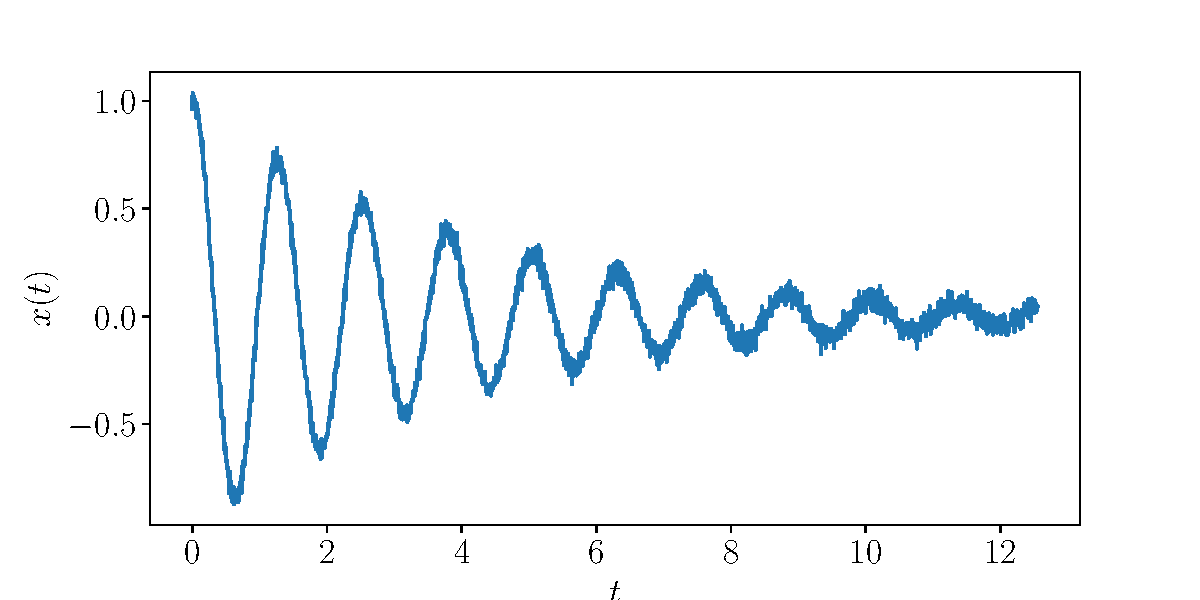
\includegraphics[scale=0.5]{nwave}
\label{f4}
\centering
\caption{The response $x(t)$ with  Gaussian noise of SNR 20.}
\end{figure}
\begin{figure}[ht]
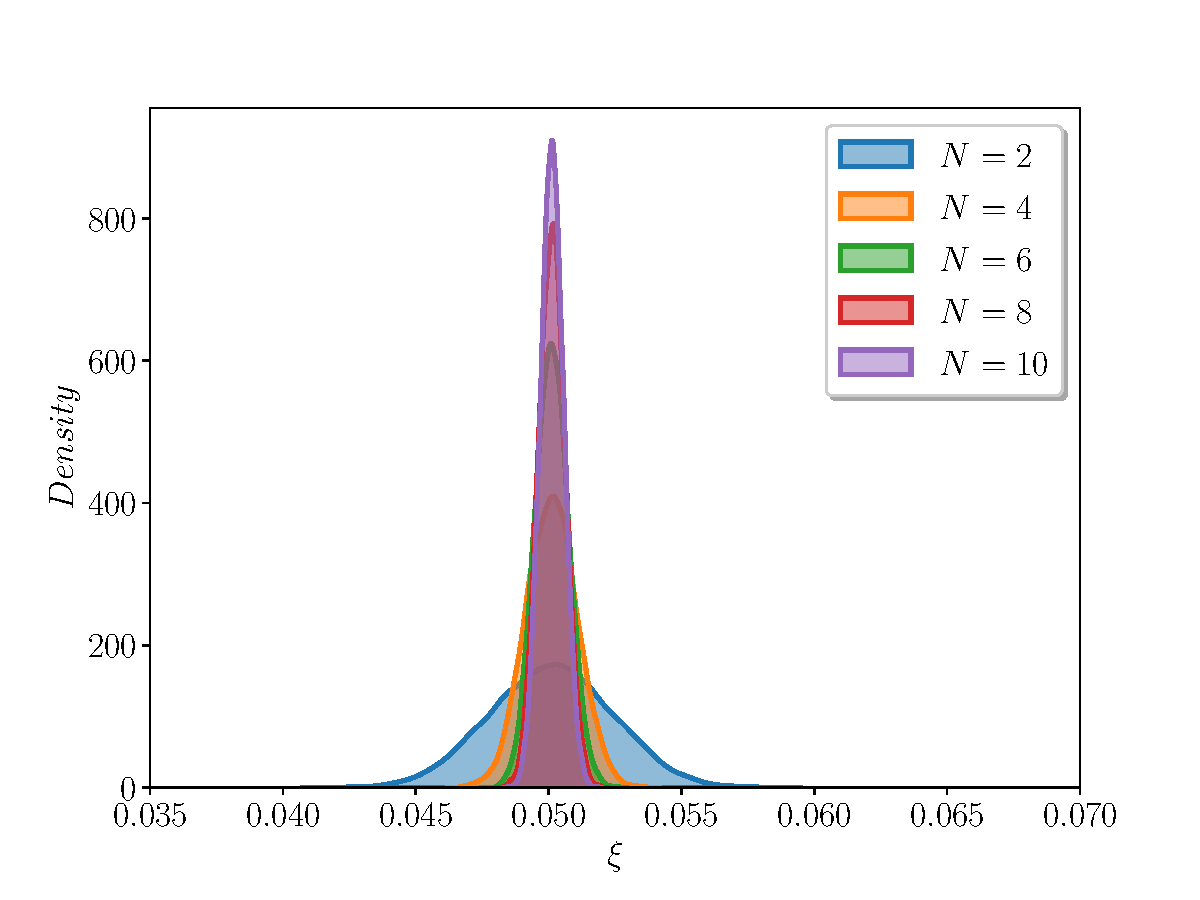
\includegraphics[scale=0.5]{fig5_1}
\label{f4}
\centering
\caption{The distribution of $\xi$ with 10000 times simulated for Gaussian noise of SNR 20 and with N.}
\end{figure}

\begin{figure}[h]
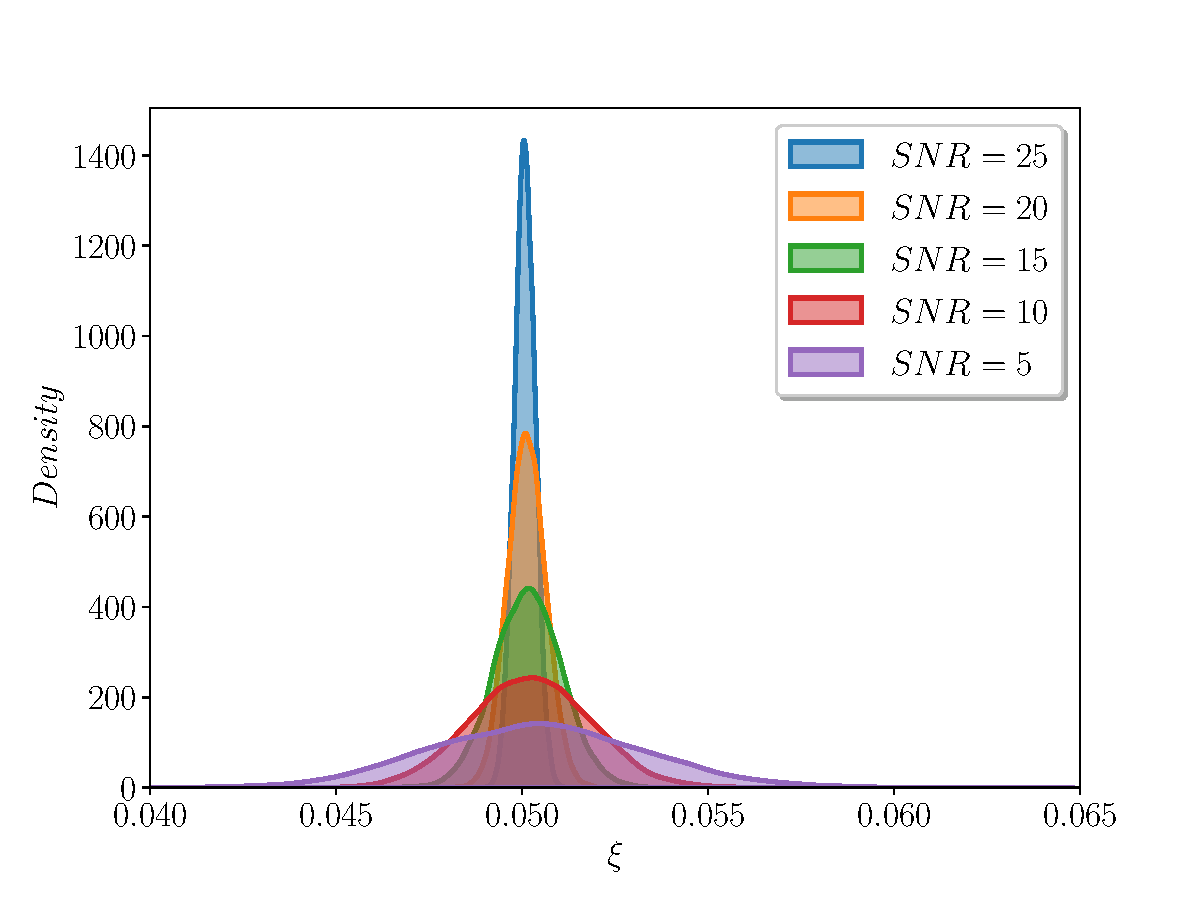
\includegraphics[scale=0.5]{fig_snrv}
\centering
\caption{The distribution of $\xi$ with 10000 times simulated for N=8 and with SNR.}
\end{figure}

From Fig.~\ref{f4} we observe that as we increase the number of areas, the error in the predicted $\xi$
becomes small after a certain number of areas, the increment in areas will not benefit much. 
This jives with our observations from the uncertainty analysis results in Fig.~\ref{uL1}. 
We also observe that as the noise increases, our prediction accuracy in $\xi$ decreases, which is expected, but the error in this analysis is less than the same system studies in ~\cite{Huang2007}. 